En este capítulo se describe el clustering y dos métodos principales. También se comentan varios métodos para elegir el número óptimo de clusters. \\

Clustering es una técnica de aprendizaje no supervisado que a partir de un conjunto de datos y una medida de similitud o distancia entre ellos los agrupa en distintas clases o clusters de forma que elementos que están en el mismo clúster son más parecidos entre ellos que con los de otro clúster distinto. \\

En primer lugar se describen los algoritmos de clustering más utilizados y posteriormente se comentarán métodos para elegir el número de clases o clusters óptimo. \\

\section{K-means}
El algoritmo de clustering K-means agrupa $n$ elementos en $k$ clusters $S_k$ con el objetivo de minimizar la suma del error cuadrático intra-cluster:

\begin{equation}
\sum_{i=1}^{k}\sum_{x\in S_i}\lVert x-\mu_{i}\rVert ^2 \nonumber
\end{equation}

donde $\mu_i$ es la media de las distancias entre los elementos en $S_i$, también conocidos como centroides. \\

La suma del error cuadrático intra-cluster o inercia es un indicador de la cohesión de los clusters. A mayor cohesión, menor distancia existirá entre los elementos de cada clúster y por tanto también del centroide. Este indicador sin embargo tiene ciertas desventajas:
\begin{itemize}
\item Asume que los clusters se modelan como esferas, al estar basado en $k$ centroides y minimizar la distancia euclídea, lo que implica misma varianza entre clusters. Ver \ref{fig_kmeans1}.
\item No es una métrica normalizada
\item Muy sensible a outliers al utilizar la distancia al cuadrado
\item No tiene en cuenta la densidad de cada cluster. Implícitamente asume que al ocupar cada clúster el mismo área cada cluster tiene que tener el mismo número de puntos. Ver \ref{fig_kmeans2}.
\end{itemize}

\begin{figure}[ht!]
\begin{center}
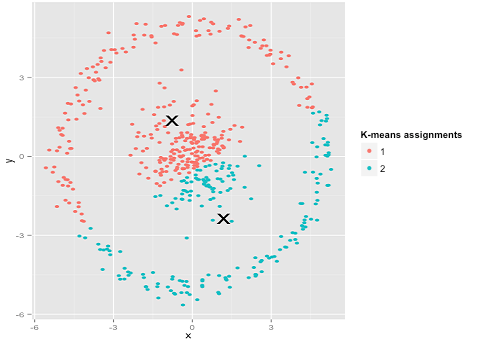
\includegraphics{figuras/kmeans1.png}
\end{center}
\caption{K-means frente a varianza en clusters}
\label{fig_muestreo}
\end{figure}

\begin{figure}[ht!]
\begin{center}
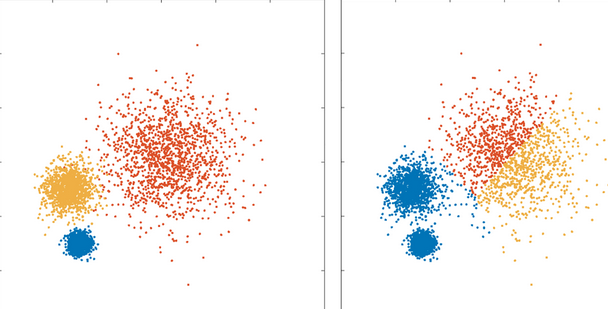
\includegraphics[width=10cm,height=10cm,keepaspectratio]{figuras/kmeans2.png}
\end{center}
\caption{K-means no es sensible a la densidad de puntos}
\label{fig_kmeans2}
\end{figure}

Dado un conjunto de $n$ elementos $\{x_1, x_2, \dots, x_n\}$ K-means empieza con una fase de inicialización en la que se escogen $k$ centroides, $\{c_1, c_2, \dots, c_k\}$. Una vez elegidos los centroides, itera de la siguiente forma: 
\begin{itemize}
\item \textbf{Etapa de asignación}: asigna cada elemento al centroide que minimiza la distancia euclídea al cuadrado, el cluster $S_i$ que tiene como centroide $c_i$ es
\begin{equation}
S_i = \{x_j : \lVert x_j - c_i \rVert ^2 \leq \lVert x_j - c_p \rVert ^2 \; \forall p, 1\leq p \leq k\} \nonumber
\end{equation}
\item \textbf{Actualización de los centroides}: serán la media de los elementos del cluster correspondiente.
\begin{equation}
c_i = \frac{1}{\displaystyle |S_i|}\sum_{x_j \in S_i}x_j \nonumber
\end{equation}
\end{itemize}

Cuando en la etapa de asignación no se producen cambios entre dos iteraciones consecutivas, el algoritmo termina. \\

La inicialización de los centroides es un aspecto muy relevante en el algoritmo: K-means converge cuando encuentra un óptimo local por lo que se han desarrollado diversos métodos de inicialización de forma que se encuentre el óptimo global:
\begin{itemize}
\item Aleatorio: se asigna de forma aleatoria un elemento a cada cluster y posteriormente se calculan los centroides en base a esta asignación. Este método ubica los centroides cerca del centro del conjunto de datos.
\item Forgy: se escogen al azar $k$ elementos del conjunto y se utilizan como centroides. Este método tiende a dispersar los centroides iniciales.
\item MacQueen: escoger al azar $k$ elementos del conjunto y tratarlos como centroides. Asigna cada elemento al cluster con el centroide más próximo y recalcula los centroides, que serán los centroides de inicialización para el algoritmo.
\item K-means++: propuesto en el a\~no 2007. Funciona de la siguiente forma:
    \begin{enumerate}
    \item Se elige un centroide elegido aleatoriamente sobre el conjunto de observaciones.
    \item Se calcula la distancia al cuadrado entre cada observación y el centroide seleccionado.
    \item Se elige otro punto al azar como segundo centroide, la probabilidad que tiene cada observación de ser elegido es proporcional a la distancia al cuadrado calculada en (2).
    \item Repetir (2) y (3) hasta tener $k$ centroides.
    \end{enumerate}
\end{itemize}

En los últimos a\~nos se ha utilizado ampliamente la inicialización mediante K-means++, además de ejecutar varias veces el algoritmo con distintos centroides para evitar óptimos locales. \\

\section{Clustering jerárquico}
El clustering jerárquico se refiere a una familia de algoritmos de clustering que construyen clusters de forma anidada al fusionarlos (clustering aglomerativo) o dividirlos (clustering divisivos). 

Cuando se trata de clustering aglomerativo, dado un conjunto de $n$ elementos cada uno constituirá un cluster y en cada iteración se fusionarán dos clústers de forma que se minimize la medida de distancia o similitud especificada, terminando el algoritmo cuando haya $1$ cluster.

En el caso de clustering divisivo, dado un conjunto de $n$ observaciones se agrupan en un único cluster y se producen sucesivas divisiones, terminando cuando haya $n$ clusters. \\

En cualquiera de los dos casos, las sucesivas iteraciones son representadas a través de un dendrograma. Como se puede ver en \ref{fig_dendrograma} un dendrograma es un diagrama en forma de árbol. En este caso muestra un algoritmo de clustering aglomerativo en el que los elementos $\{a, b, c, d, e, f\}$ se han ido agrupando en sucesivas iteraciones hasta terminar con $1$ cluster. \\

\begin{figure}[ht!]
\begin{center}
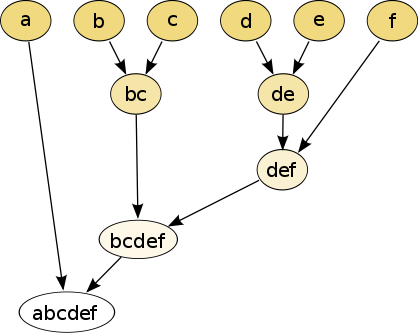
\includegraphics[width=10cm,height=10cm,keepaspectratio]{figuras/dendrograma.png}
\end{center}
\caption{Dendrograma\cite{wiki:dendrogram}}
\label{fig_dendrograma}
\end{figure}

En lo sucesivo se contemplará el clustering aglomerativo, los conceptos y métodos para el caso divisivo son análogos. Para decidir cómo agrupar los clusters de forma iterativa es necesario definir una medida de similitud entre clusters, de forma que clusters similares se agrupen antes que clusters distintos. En la primera iteración en la que todos los clusters están compuestos por un único elemento se puede especificar una distancia, en el resto de iteraciones será necesario definir un criterio de enlace o \textit{linkage criteria} que modele cómo medir la similitud entre dos clusters en los que al menos uno de ellos está compuesto por más de una observación. \\

Se puede especificar cualquier distancia $d$, mientras cumpla las propiedades de distancia desde un punto de vista matemático, que son:
\begin{itemize}
\item $d(x,y) \geq 0$ y $d(x,y)=0 \iff x=y$
\item $d(x,y) = d(y,x)$ o propiedad simétrica
\item $d(x,z) \leq d(x,y) + d(y,z)$ o desigualdad triangular
\end{itemize}

Las distancias más habituales son las siguientes:
\begin{itemize}
\item Distancia euclídea. La más común y la que se utiliza por defecto.
    \begin{equation}
    d(x,y) = \sqrt{\sum(x_i-y_i)^2} \nonumber
    \end{equation}
\item Distancia del taxi, también conocida como distancia Manhattan debido al dise\~no en cuadrícula de las calles de la isla.
    \begin{equation}
    d(x,y) = \sum |x_i - y_i| \nonumber
    \end{equation}
\item Distancia de Chebyshev, también conocida como distancia del tablero de ajedrez ya que coincide con el número de movimientos que necesita el rey para moverse de una casilla a otra.
    \begin{equation}
    d(x,y) = \max{|x_i - y_i|} \nonumber
    \end{equation}
\item Distancia de Hamming, para vectores lógicos, es el número de bits que tienen que cambiarse para transformar un vector de bits en otro.
    \begin{equation}
    d(x,y) = \frac{\displaystyle c_{01} + c_{10}}{\displaystyle n} \nonumber
    \end{equation}
donde $c_{ij}$ es el número de ocurrencias de $x[k] = i, y[k] = j$ para $k < n$. 
\item Distancia de Mahalanobis. Distancia muy útil para determinar la similitud entre dos variables aleatorias multidimensionales al tener en cuenta la correlación y la escala de ellas.
    \begin{equation}
    d(x,y) = \sqrt{(x-y)V^{-1}(x-y)^T} \nonumber
    \end{equation}
donde $V$ es la covarianza y $V^{-1}$ la inversa de la matriz de covarianza.
\end{itemize}

Además, otras que son ampliamnete utilizadas son Bray-Curtis, Canberra, coseno, Minkowski, o la euclídea normalizada. Para el caso de variables booleanas, además de la ya mencionada arriba distancia Hamming se han empleado: dado, Jaccard-Needham, Kulsinski, Rogers-Tanimoto, Russell-Rao, Sokal-Michener, Sokal-Sneath y Yule. \\

Una vez definidas la distancia a utilizar entre cada par de observaciones, se pueden definir distintos criterios de enlace entre dos clústers $u$ y $v$. Los más habituales son los siguientes:
\begin{itemize}
\item Método \textit{single} o del punto más cercano. 
    \begin{equation}
    d(u,v) = \min{(dist(u[i], v[j]))} \nonumber
    \end{equation}
para todos los puntos $i$ en el cluster $u$ y todos los $j$ en $v$. Este algoritmo se centra en la separación entre clusters pero no en la cohesión de los clusters y permite formas geométricas más flexibles que en otros casos.
\item Método \textit{complete}, también conocido como Algoritmo del punto lejano o Algoritmo de Voor Hees.
    \begin{equation}
    d(u,v) = \max{(dist(u[i], v[j]))} \nonumber
    \end{equation}
\item Método \textit{average} o algoritmo UPGMA.
    \begin{equation}
    d(u,v) = \sum_{ij}\frac{\displaystyle dist(u[i], v[j])}{(|u| * |v|)} \nonumber
    \end{equation}
\item Método \textit{weighted} o algoritmo WPGMA,
    \begin{equation}
    d(u,v) = (dist(s,v) + dist(t,v))/2
    \end{equation}
donde el cluster $u$ está compuesto por los clusters $s$ y $t$.
\item Método \textit{centroid} asigna como distancia entre clusters la distancia euclídea entre sus centroides.
\item Método \textit{ward}. Según Ward la distancia entre dos clusters $u$ y $v$ es el incremento que se producirá en la suma del error cuadrático si se fusionan:
    \begin{equation}
    d(u,v) = \sqrt{\frac{|v|+|s|}{T}d(v,s)^2 + \frac{|v|+|t|}{T}d(v,t)^2 - \frac{|v|}{T}d(s,t)^2}
    \end{equation}
donde $u$ es el nuevo cluster creado a partir de $s$ y $t$ y $T=|v|+|s|+|t|$. En este caso, a diferencia de K-means, el número de puntos interviene en la fórmula por lo que dados dos pares de clusters cuyos centros están distanciados por igual, el algoritmo de Ward fusionará los de menor cardinalidad.
\end{itemize}

\section{Elección del número de clusters óptimo}
Los algoritmos de clustering se utilizan principalmente de dos propósitos distintos según la problemática:
\begin{itemize}
\item Se conoce a priori el número de distintas clases en la población y se quieren obtener los cortes en el vector de características de las observaciones para conocer qué características tiene cada clase. Nuevas observaciones podrán ser categorizadas a partir del conocimiento extraído en el clustering.
\item No se conoce cuántas clases distintas existen en la población y se quiere conocer esto a partir del clustering.
\end{itemize}

Es en el segundo caso en el que no se tiene información sobre el $k$ a utilizar en el algoritmo K-means o el corte a aplicar en el dendrograma en clustering jerárquico. En lo que sigue se describen distintos métodos basados en heurísticas para determinar el número de clusters óptimo. \\

\subsection{Coeficiente silueta}
Para cada observación $x$ se tienen dos medidas:
\begin{itemize}
\item Cohesión $a(x)$: grado de similitud del elemento respecto del cluster. Se obtiene como la distancia promedio de $x$ a todos los puntos en el mismo cluster. 
\item Separación $b(x)$: grado de disimilitud del elemento respecto a elementos que han sido identificados en otras clases. La separación más utilizada es la distancia promedio entre $x$ y todos los elementos del cluster más cercano, aunque también se utilizan otras medidas para valorar la separación.
\end{itemize}

El coeficiente silueta para $x$ se define entonces como
\begin{equation}
s(x) = \frac{\displaystyle b(x) - a(x)}{\displaystyle \max{\{a(x), b(x)\}}} \nonumber
\end{equation}

y para todo el agrupamiento es
\begin{equation}
SC = \frac{1}{n}\sum_{x}s(x)
\end{equation}

donde $n$ es el número de observaciones. \\

Intuitivamente, un agrupamiento bien definido debería corresponderse con que para cada elemento $x$ se tiene que $a(x) << b(x)$, es decir, $x$ está muy cercano respecto de los elementos de su cluster en comparación con los elementos del cluster más cercano. El coeficiente $s(x)$ toma los valores en el rango $\left[ -1, 1\right]$, donde $-1$ corresponde con una mala elección del número de clusters y $1$ indica clusters bien definidos. \\

De esta forma, una de las técnicas que se usa con el coeficiente silueta es elegir un rango de valores para $k$, y elegir $k$ de forma que el coeficiente silueta para el agrupamiento sea máximo.

\subsection{Índice Calinski-Harabasz}
Dado $k$, se define el índice de Calinski-Harabasz como:
\begin{equation}
s(k) = \frac{SS_B}{SS_W} * \frac{N-k}{k-1} \nonumber
\end{equation}
$SS_B$ es la varianza entre clusters
\begin{equation}
SS_B = \sum_{i=1}^{k}n_id(m_i, m)^2 \nonumber
\end{equation}
donde $m_i$ es el centroide del cluster $i$ y $m$ es la media de todas las observaciones.

$SS_W$ es la varianza intra-cluster:
\begin{equation}
SS_W = \sum_{i=1}^{k}\sum_{x\in S_i}d(x, m_i)^2 \nonumber
\end{equation}

Para que los clusters estén bien definidos deben tener valores grandes para $SS_B$ (medida de separación) y peque\~nos para $SS_W$ (medida de cohesión). De esta forma el índice de Calinski-Harabasz es una adaptación del método F-test de ANOVA, $SS_B$ con $k-1$ y $SS_W$ con $n-k$ grados de libertad por lo que aparecen en la fórmula pues $SS_B$ debe ser proporcional a $k-1$ y $SS_W$ proporcional a $n-k$.  \\

El método a seguir es el mismo que en el caso del coeficiente silueta, elegir un rango de valores para $k$ y elegir el $k$ que maximice el coeficiente Calinski-Harabasz. \\

Al igual que el coeficiente silueta, es un método que funciona generalmente bien para clusters convexos.

\subsection{Método del codo}
El método del codo consiste en representar en una gráfica el porcentaje de varianza explicada frente al valor $k$ del número de clusters. De forma visual se identifica el valor de $k$ como aquel que si se a\~nadiese otro cluster no mejora o incrementa apenas la varianza explicada. \\

Cabe mencionar que el método del codo no está ligado únicamente a la varianza explicada y pueden utilizarse otras medidas como por ejemplo en clustering jerárquico la distancia mínima entre clusters en cada iteración. En ese caso las distancias serán peque\~nas hasta que en un punto aumenten considerablemente al fusionar clusters muy distintos. Este último punto será el $k$ óptimo buscado. \\

Este método recibe el nombre por la gráfica característica que se produce al representar una de estas variables frente al número de clusters, como puede verse en \ref{fig_elbow}, donde el $k$ óptimo aparece marcado en rojo. \\

\begin{figure}[ht!]
\begin{center}
\includegraphics[width=10cm,height=10cm,keepaspectratio]{figuras/elbow.png}
\end{center}
\caption{Método del codo}
\label{fig_elbow}
\end{figure}

\subsection{Método Gap}
El método Gap fue desarrollado por unos investigadores en Stanford\cite{gap:2001}. Este método formaliza matemáticamente el método del codo para encontrar el $k$ óptimo. Dado 
\begin{equation}
W_k = \sum_{r=1}^{k}\frac{\displaystyle 1}{\displaystyle 2n_r}D_r \nonumber
\end{equation}
donde $D_k$ es la suma de la distancia intra-cluster entre sus elementos. En caso de utilizarse la distancia euclídea, $W_k$ es la suma de los cuadrados de las distancias intra-cluster. \\

La idea es estandarizar el gráfico $\log{(W_k)}$ mediante la comparación de este con su esperanza bajo una distribución nula de referencia. Se define por tanto el estadístico Gap como
\begin{equation}
Gap_n(k) = E_n^*\{\log{(W_k)}\} - \log{(W_k)} \nonumber
\end{equation}

El valor óptimo de $k$ es el mínimo $k$ tal que $Gap(k) \geq Gap(k+1) - s_{k+1}$, donde $s$ es la desviación mínima. En \ref{fig_gap} se muestra la similitud entre el método del codo y el de Gap. \\

\begin{figure}[ht!]
\begin{center}
\includegraphics[width=10cm,height=10cm,keepaspectratio]{figuras/gap.png}
\end{center}
\caption{Método del codo y método Gap}
\label{fig_gap}
\end{figure}
